\section{Phase 3}

安全審査 Phase III では,FM検証試験結果までのシステム安全検証の妥当性に
ついて評価を受けた.審査自体は文書審査となり, 代わりに事前確認会が実施
された.プロジェクトメンバーからは,坂本,中西,池谷,井出,大本が
Polycom 遠隔会議システムにより東工大より参加した.

\subsection{Phase II からの変更点}
Phase II からの変更点を表\ref{5_3_def}に示す.安全審
査の適用範囲が変更されたため,構造に関するハザードが審
査対象外となり,提出文書から UHR-1, UHR-2が除外となった点が特に大きな
変更となっている.

\begin{table}[htbp]
\centering
	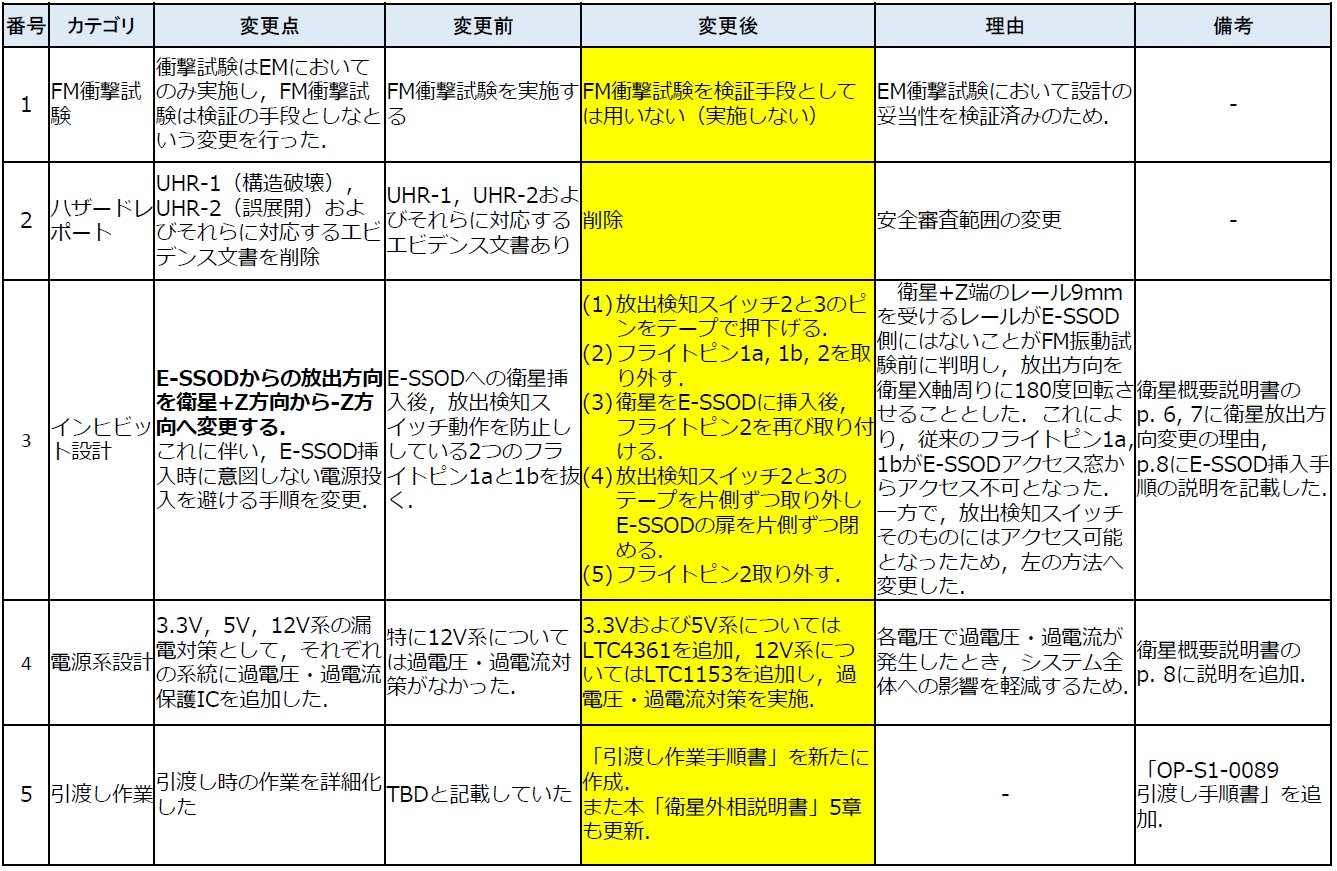
\includegraphics[width=14cm]{./05/fig/5_3_def.jpg}
	\caption{Phase II からの変更点}
	\label{5_3_def}
\end{table}

\subsection{審査結果}
各システム安全文書について対処・検証結果は適切であるとの判定を受けた.
しかし,審査直前に発生した不具合により再組立てが発生したため,
OP-S1-0103 OrigamiSat-1 FM 再組立て記録の提出および OP-S1-0035 インヒ
ビット確認試験報告書の再提出がA/Iとなり,これらの提出を持って審査が完
了となった.

\subsection{審査後の安全検証追跡ログ (VTL) について}
本審査後の安全検証結果については,OP-S1-0090 OrigamiSat-1 安全検証追跡
ログ にて,管理を実施した.
